\subsection{Part Selection}
In our research for part selection we wanted to create a generalized comparison of the options we have available. We formatted this information in the tables below.

\subsubsection{Controller Subsystem}
\paragraph{Minimum Requirements} At minimum, any chosen microcontrollers (MCUs) shall support natively, or by addition of a module, these features and traits:
\begin{itemize}
	\item Ability to connect to external antenna
	\item Analog-to-digital converter (ADC)
	\item IEEE 802.11
	\item In stock and available to order
	\item JTAG module or equivalent
	\item Module communication bus (UART, I2C, SPI)
	\item Network stack
	\item Onboard CPU sufficient for our purposes
	\item Onboard memory sufficient for our purposes
	\item Onboard nonvolatile memory
	\item Sockets support
	\item Pins dedicated to analog input
	\item Pins dedicated to digital I/O
\end{itemize}

\paragraph{Nice To Have} These features would be "nice to have" on any MCU selected, but are not required:
\begin{itemize}
	\item Digital-to-analog converter (DAC)
	\item Integrated antenna
	\item microSD card slot
	\item Onboard battery
	\item Pins dedicated to pulse-width modulation (PWM)
	\item Timer(s) and an RTC
	\item USB compatibility
	\item Additional wireless communication protocols (e.g. BT or BLE, Zigbee)
\end{itemize}

\paragraph{Selections} The selections, listed in \autoref{table:mcubreakdown1} and not in any particular order, match the above criteria and are being considered for selection.
\begin{table}
	\centering
	\begin{tabularx}{\textwidth}
		{
			| >{\raggedright\arraybackslash}X
			| >{\raggedright\arraybackslash}X
			| >{\raggedright\arraybackslash\columncolor[gray]{0.8}}X
			| >{\raggedright\arraybackslash}X
			| >{\raggedright\arraybackslash}X
			| >{\raggedright\arraybackslash}X
			|
		}
		\caption{MCU option breakdown}
		\label{table:mcubreakdown1} \\
		\hline
		\textbf{Model} & \textbf{\href{https://www.ti.com/tool/LAUNCHXL-CC26X2R1}{LAUNCH\-XL-CC26X2\-R1}} & \textbf{\href{https://www.ti.com/tool/LAUNCHCC3220MODASF}{LAUNCH\-CC3220\-MODASF}} & \textbf{\href{https://www.raspberrypi.com/products/raspberry-pi-pico/}{Pico W}} & \textbf{\href{https://store-usa.arduino.cc/products/arduino-nano-33-ble?selectedStore=u}{Nano 33 BLE}} & \textbf{\href{https://www.st.com/en/evaluation-tools/b-l4s5i-iot01a.html}{B-L4S5I-IOT01A}} \\
		\hline
		\textbf{Manu\-facturer} & Texas Instruments & Texas Instruments & Raspberry Pi & Arduino & STMicro\-electronics \\
		\hline
		\textbf{Micro\-controller} & CC2652R & CC3220\-MODASF & RP2040 & nRF52840 & STM32\-L4S5VIT6 \\
		\hline
		\textbf{Processor} & 1x ARM Cortex-M4F & 1x ARM Cortex-M4 & 2x ARM Cortex-M0+ & 1x ARM Cortex-M4 & 1x ARM Cortex-M4 \\
		\hline
		\textbf{Maximum Speed (MHz)} & 48 & 80 & 133 & 64 & 120 \\
		\hline
		\textbf{Memory (KB)} & 256 ROM, 352 flash, 100 SRAM & 1024 flash, 256 RAM & 16 ROM, 264 SRAM & 1024 flash, 256 SRAM & 2048 flash, 640 RAM \\
		\hline
		\textbf{Wireless capability} & BLE5.2, Zigbee, Thread & 802.11b/g/n & 802.11n & BLE5.3, Zigbee, Thread, Matter & BT4.1, 802.11b/g/n, NFC \\
		\hline
		\textbf{Serial capability} & UART, I2C, I2S, SPI & UART, I2C, SPI & UART, I2C, SPI, USB1.1 & UART, I2C, I2S, SPI, USB2.0 & UART, I2C, SPI, USB2.0 \\
		\hline
		\textbf{Price (\$)} & 40, maybe free & 60, maybe free & 6 & 28 & 53 \\
		\hline
		\textbf{ADC} & 8-channel, 12-bit & 4-channel, 12-bit & 4-channel, 12-bit & 8-channel, 12-bit & 16-channel, 12-bit \\
		\hline
		\textbf{Watchdog timer?} & No & Yes & Yes & Yes & Yes \\
		\hline
		\textbf{GPIO (pins)} & 31 & 29 & 30 & 13 & 16 \\
		\hline
		\textbf{PWM (channels)} & Supported & Supported & 16 & 4 & 6 \\
		\hline
		% \textbf{AES (bits)} & 128, 256 & 256 & Not supported & 128 & 128 \\
		% \hline
		\textbf{Required voltage (V)} & 1.8 -- 3.8 & 2.3 -- 3.6 & 1.8 -- 3.3 & 4.5 -- 21 & 4.75 -- 5.25 \\
		\hline
	\end{tabularx}
\end{table}

\paragraph{Single-board Computers} Use of single-board computers (SBCs) was considered, but will not not need to be used; sockets will be used on an MCU in conjunction with \href{https://aws.amazon.com/ec2/}{Amazon EC2} services will allow us to offload computing to a cloud solution.

\paragraph{External WiFi Module} Use of an external WiFi module is discouraged due to the following reasons:
\begin{itemize}
	\item Added cost
	\item Added complexity
	\item Modules in common use by hobbyists often have poor or no proper documentation, to the
	extent of:
	\begin{itemize}
		\item Quick start guide
		\item User's guide
		\item Datasheets
		\item Theory of operation
		\item Application uses
		\item Troubleshooting guide
		\item Schematics and mechanicals
		\item Quality and reliability
		\item Errata
	\end{itemize}
\end{itemize}
Therefore, all of the MCUs listed above support either the 802.11 or Bluetooth standards.

\paragraph{External ADC Module} Use of an external ADC was considered, but ultimately decided against. An external ADC module would only add further cost and complexity to a project where the on-chip ADC is sufficiently effective for the project's requirements. The sample rate and resolution of an on-chip ADC is more than enough for our needs, and the low-cost goal of the project directly conflicts with the idea of purchasing an external ADC module.

\paragraph{Selection} Ultimately, the \href{https://www.ti.com/tool/LAUNCHCC3220MODASF}{LAUNCHCC3220MODASF} was chosen as the microcontroller development board for this project. In the event that the aforementioned LaunchPad is not able to be obtained, the \href{https://www.ti.com/tool/CC3220SF-LAUNCHXL}{CC3220SF-LAUNCHXL} has  quivalent capability for the project's needs.

These boards, henceforth referred to as the CC3220, are able to be requested from our university at no upfront cost to our team. This was the driving factor behind choosing the CC3220 over other microcontroller development boards. It was also determined that the microcontroller \emph{must} be able to interface via the 802.11 (WiFi) standard, for reasons that are detailed in \autoref{sec:controller_subsystem}---therefore, the LAUNCHXL-CC26X2R1 and Nano 33 BLE were disqualified from selection. The Pico W was considered due to its low cost, and the B-L4S5I-IOT01A considered because of its abundant peripherals, but both ultimately lost out to the Texas Instruments products.

\paragraph{CC3200} Due to difficulties in acquiring the CC3220 (second-generation SimpleLink device), our team made the decision to use the CC3200 (first-generation SimpleLink). These parts are mostly identical, with the differences detailed in \autoref{table:cc32x0_diff}. Development will take place on the \href{https://www.ti.com/tool/CC3200-LAUNCHXL}{CC3200-LAUNCHXL}, with the PCB MCU part to be \href{https://www.ti.com/product/CC3200}{CC3200} (if needed).

\begin{table}
	\centering
	\begin{tabularx}{\textwidth}
		{
			| >{\raggedright\arraybackslash}X
			| >{\raggedright\arraybackslash\columncolor[gray]{0.8}}X
			| >{\raggedright\arraybackslash}X
			|
		}
		\caption{Differences between CC3200 and CC3220}
		\label{table:cc32x0_diff} \\
		\hline
		\textbf{Model} & \textbf{CC3200} & \textbf{CC3220} \\
		\hline
		\textbf{Micro\-controller} & CC3200 & CC3220SF \\
		\hline
		\textbf{Secure Flash (MB)} & n/a & 1 \\
		\hline
		\textbf{Simultaneous TCP/UDP Sockets} & 8 & 16 \\
		\hline
		\textbf{WiFi Receive Sensitivity (dBm, 1 DSSS)} & -95.7 & -96 \\
		\hline
		\textbf{WiFi Receive Sensitivity (dBm, 54 OFDM)} & -74.0 & -74.5  \\
		\hline
		\textbf{Hibernate Current Draw ($\upmu$A)} & 4 & 4.5  \\
		\hline
		
	\end{tabularx}
\end{table}

\paragraph{Bill of Materials} The bill of materials for the controller subsystem can be found in \autoref{table:controller_bom}.

\begin{table}
	\centering
	\begin{tabularx}{\textwidth}
		{
			| >{\raggedright\arraybackslash}l
			| >{\raggedright\arraybackslash}l
			| >{\raggedright\arraybackslash}X
			| >{\raggedright\arraybackslash}X
			| >{\raggedright\arraybackslash}X
			|
		}
		\caption{Controller subsystem bill of materials}
		\label{table:controller_bom} \\
		\hline
		\textbf{Qty} &  \begin{tabular}[c]{@{}l@{}}\textbf{Cost}\\\textbf{(\$/ea)}\end{tabular}& \textbf{Manufacturer} & \textbf{Item} & \textbf{Model Number} \\
		\hline
		1 & 0.00 & Texas Instruments & SimpleLink Wi-Fi CC3200 LaunchPad & CC3220-LAUNCHXL \\
		\hline
		2 & 10.88 & Texas Instruments & CC3200 & CC3200R1M2RGCR \\
		\hline
		2 & 3.80 & Taiyo Yuden & Surface Mount 2.4 GHz Antenna & AH316M245001-T \\
		\hline
		2 & 6.95 & Adafruit & Plastic Water Solenoid Valve & 997 \\
		\hline
	\end{tabularx}
\end{table}




% End Controller Subsystem

\subsubsection{Power Subsystem}
\paragraph{Power Supply}
The power system is a key factor to this model and trying to make this an independent system. This is key because this power system needs to be able to power all of the many different components, while also charging itself when not operating.

As part of the goal to make this an independent system, solar energy plays a great role in this and making this system run. Before anything as well, this part of the system must operate first before it can power other components. For this system to run, the key parts include: solar panels that convert light energy into electrical energy; solar charge controller to regulate output voltage from the solar panel into the battery; the battery to directly power the other components in the model.

In this model there are many different sensors, electrical, and mechanical components all of which require power. This requires a design of how the power system will flow and operate. It first begins with determining the total power needed for the whole system to run. This can be determined by finding the individual power ratings of each component and calculating them all together. After that is found, we can then choose what type of battery and the quantity needed for the model. When choosing what kind of battery and how many is needed, how long we want the system to run, optional secondary power source, and optional battery bank must be put into consideration as well. As follows, we begin to research solar panels from type, efficiency, power rating, etc. Then, a solar charge controller must be selected, a device that sits between the solar panel and the battery to regulate how much power is going into the battery. Once that is done, a voltage regulator must be determined, to regulate voltage from the battery to the smaller components that need to be powered. After all that is done, then we can find other components that will make the power system more reliable and efficient in any way.

\paragraph{Power Requirement}
Sensors, electrical, and mechanical components all require power but all consume different amounts of power. As mentioned before, analyzing the total power requirement is important and crucial because this will help us determine the right parts that will be best for this system and for the components.

With the total power determined, the Watts per hour needed for all of the components to run must also be found. The watts per hour is important too because this helps figure out how long each component will operate for. After that is found, we used the altE calculator to help pick out what kind of battery can be used, then solar panel and solar charge controller, respectively. The altE calculator is a great resource because with the proper measurements, it can help us choose what kind of battery we can use, by determining the capacity needed in watt-hours or amp-hours. This calculator can also help us choose how big of a solar panel we need and how big of a solar charge controller we need as well.
\paragraph{Rechargeable Battery Selection}
Solely relying on solar energy isn’t always ideal. This is because the weather may not always guarantee sunlight, this will hinder its power retention. For this reason, solar panels are paired with a battery so that the power can be stored and then used at a later time. As part of the goal to have this run as an independent system, an additional battery may be used so that one battery can power the system while the other one can charge.

There are many different types of batteries including Nickel-Cadmium, Nickel-Metal Hydride, Lithium ion, etc. Of the three batteries, they will be compared to see which will best fit our model and which will fulfill the requirements on the basis of power output, efficiency, etc.

Nickel Cadmium (NiCd) batteries in today’s time are used for RC vehicles, power tools, photography equipment, and more. They would also be considered as old technology. Even though they are old, they still have their advantages such as being less expensive, they are super powerful and charge fast, they require little maintenance, and more. These batteries though also has its disadvantages, one being they suffer from “ memory” problems and as a result of that, it may reduce that capacity of charges and future battery life. These batteries are also environmentally concerning because cadmium is toxic.

Nickel-Metal Hydride (NiMH) is similar to nickel cadmium, the only difference is that hydrogen is used instead of cadmium as the active element. Hybrid cars, toothbrushes, and phones are just a few of many products that use nickel-metal hydride batteries and have been used in these appliances because of the trouble free service they grant. It is also because even being partially discharged, it can be charged as many times and will always be at full capacity. Even with advantages like that nickel-metal hydride batteries produce a lot of heat when in use, have a high self-discharge rate, and have memory issues as well, just not as bad as NiCd.

Lithium ion batteries, one of the most popular types of rechargeable batteries for portable products. It is considered the best because lithium ion batteries have high open circuit voltage, low self-discharge rates, and little to no memory effect. On top of that they are growing within the military, electric vehicle companies, and aerospace industry with little to no maintenance. Even though they have a lot of advantages, some of the disadvantages include sensitivity towards high temperatures, it cannot be fully discharged, and the cost.

Through much consideration and investigation, the four batteries listed in the following table were picked. All of which are 12V lithium iron phosphate (LiFePO4) batteries. Then the selected battery that we decided we were going to use for this model is the Eco Worthy 12V 8Ah LiFePO4 battery. We decided to go with this battery because although it is a little expensive,the Watts per hour and the Ah rating that this battery provides, was great for what we plan on having.

\begin{table}[H]
    \centering
	
	\begin{tabularx}{\textwidth}
		{
			| >{\raggedright\arraybackslash}X
			| >{\raggedright\arraybackslash}X
			| >{\raggedright\arraybackslash}X
			| >{\raggedright\arraybackslash}X
			| >{\raggedright\arraybackslash}X
			|
		}
		\caption{Battery Selection}
		\label{table:rechargeablebatteryl} \\
		\hline
		\textbf{Manu\-facturer} & \textbf{Ampere Time} & \textbf{Eco Worthy} & \textbf{Expert\-Power} & \textbf{Eco Worthy} \\
		\hline
		\textbf{Voltage} &  12 & 12 & 12 & 12 \\
		\hline
		\textbf{mAh} &  6000 & 10000 & 5000 & 8000 \\
		\hline
		\textbf{Watt per hour} & 76.8 & 120 & 64 & 96 \\
		\hline
		\textbf{Cost} & \$29.99 & \$59.99 & \$35.99 & \$43.99 \\
		\hline
	\end{tabularx}
\end{table}
\paragraph{Solar Panel Selection}
Solar has been a growing source of energy in the past years, with new developments and breakthroughs with solar cell technology. As the whole purpose of solar energy is to collect sunlight and convert it into electrical energy, that is the minimum for this model to run as an independent system. Then as a stretch goal, we would apply the concept of solar tracking panels to create blinds with the solar panels so it can open and close according to the position of the sun.

On a basic level, solar panels are made of solar cells and these cells do the collecting and converting. These solar cells are made from crystalline silicon that is melted down into ingots and then cut into sheets. In the solar industry there are 3 main types of solar panels. These types of panels are monocrystalline, polycrystalline, and thin-film panels all of which have different compositions. Each type has different efficiencies, generating different amounts of power, etc.

Monocrystalline solar panels are solar panels that are made with monocrystalline solar cells. These solar cells are composed of a single silicon crystal which provides electrons more space to move because of the electricity flow that is generated. This makes them more efficient, yet at the same time more costly. Polycrystalline solar panels are solar panels that are made with polycrystalline solar cells. Similar to monocrystalline solar cells, they are made of a silicon crystal, the only difference is that instead of a single crystal, they use several fragments of silicon to form an ingot and that is cut into sheets. As a result of melting several fragments into one it creates a mosaic look as well as giving it a blue hue, whereas the monocrystalline solar panel will have a uniform color and look. Aesthetically, they might look nicer but they are less efficient than monocrystalline solar panels. This also means that they aren’t going to be as pricey compared to the monocrystalline panels because of the efficiency and manufacturing process. Thin-film solar panels differ from crystalline solar panels greatly, all because they are made with different materials. The three main types of thin-film solar panels are amorphous silicon (a-Si), cadmium telluride (CdTe), and copper indium gallium selenide (CIGS). Currently, thin-film solar panels are the least efficient, costly, and have the shortest lifespan. It is predicted that they will have a major growth in the solar industry because although they are the least efficient, they have a higher theoretical efficiency than both monocrystalline and polycrystalline.

The choice of solar panels will be based on multiple aspects of each type of solar panel. As we know, the efficiency rating and cost from most to least will go from monocrystalline, polycrystalline, and thin-film, respectively, but we must also look at its temperature coefficient, power rating, and more to be able to determine which solar panel we exactly need. Temperature coefficient for solar panels is the power lost as the temperature rises. This plays a very important role because we live in Florida, temperatures can get hot. So, when it comes to which solar panel will still be more efficient in higher temperatures, monocrystalline solar panels are still the best. As follows, it then goes from polycrystalline and then thin-film. This doesn’t mean we shouldn’t count them out though, because depending on where you live the temperatures may not be high so it won’t impact it as much. It could also be more cost efficient as well because the other two types of solar panels are less expensive. Another factor to keep in mind is the power capacity of each solar panel type. For monocrystalline solar panels, because of their single crystal structure it allows for a higher power output, compared to polycrystalline, its power output capacity isn’t as high. For thin-film panels, because they don’t have uniform sizes, they won’t have a standard for power capacity.


\begin{table}[H]
    \centering
	
	\begin{tabularx}{\textwidth}
		{
			| >{\raggedright\arraybackslash}X
			| >{\raggedright\arraybackslash}X
			| >{\raggedright\arraybackslash}X
			| >{\raggedright\arraybackslash}X
			|
		}
		\caption{Solar panel types}
		\label{table:solarpanel} \\
		\hline
		\textbf{Solar Panel Type} & \textbf{Mono\-crystalline} & \textbf{Poly\-crystalline} & \textbf{Thin - Film} \\
		\hline
		\textbf{Efficiency} &  \textgreater20\% & 15 - 17\% & 6 - 15\% \\
		\hline
		\textbf{Power Rating} &  $\le$300W & 240 - 300W & Indefinite \\
		\hline
		\textbf{Performance} & Most efficient & Efficient & Least efficient \\
		\hline
		\textbf{Temperature} & High Tolerance & Low Tolerance & High Tolerance \\
		\hline
		\textbf{Cost per Watt} & \$1 - \$1.50 & \$.70 - \$1 & \$.43 - \$.70 \\
		\hline
	\end{tabularx}
\end{table}
Through research and investigation, different solar panels were compared to see which would be best fit for our model. With the different types of solar panels, we didn’t specifically choose what kind of solar panel type we wanted to go with because they all were great options and benefited in various ways. Of the four choices listed in the following table though, the monocrystalline solar panel was a popular type. These solar panel choices that were picked, all have a power rating of 10 Watts and a voltage rating of 12V, except for the Voltaic solar panel which was 18V. \par
The selected solar panel that we chose was the Eco Worthy 10W 12V monocrystalline. There were a lot of factors that went into this choice, one of them was because of the cost of the solar panel, it was a great price for what we were getting. It was also because of the size and weight, it makes it very easy to move around. Also, it had many great reviews and is available on different websites to order.\par
\begin{table}[H]
    \centering
	\caption{Solar panel part breakdown}
	\label{table:solarpanelparts}
	\begin{tabularx}{\textwidth}
		{
			| >{\raggedright\arraybackslash}X
			| >{\raggedright\arraybackslash}X
			| >{\raggedright\arraybackslash}X
			| >{\raggedright\arraybackslash}X
			| >{\raggedright\arraybackslash}X
			|
		}
		\hline
		\textbf{Sku} & P108 & L02M10-1 & NPA10S-12H & SLP010-12U \\
		\hline
		\textbf{Manu\-facturer} & \textbf{Voltaic Systems} & \textbf{Eco Worthy} & \textbf{Newpowa} & \textbf{SolarLand} \\
		\hline
		\textbf{Solar Panel Type} & Monocrystalline & Monocrystalline & Monocrystalline & Polycrystalline \\
		\textbf{Dim\-ensions} & 10.9 x 8.8 x .16 & 13.3 x 8.1 x .7 & 14.37 x 7.68 x .91 & 14.06 x 11.89 x 1.18 \\
		\hline
		\textbf{Peak Current} & 570mA & 580mA & 630mA & 580mA \\ 
		\hline
		\textbf{Open Circuit Voltage} & 20.45V & 20.6V & 19.83V & 21.6V \\
		\hline
		\textbf{Peak Voltage} & 17.34V & 17.3V & 16.77V & 17V \\
		\hline
		\textbf{Wattage} & 9 watt & 10 watt & 10 watt & 10 watt \\
		\hline
		\textbf{Power Tolerance} & $\pm$10\% & $\pm$3\% & $\pm$3\% & $\pm$5\% \\
		\hline
		\textbf{Cost} & \$49 & \$25.99 & \$25.99 & \$35.53 \\
		\hline
	\end{tabularx}
\end{table}
\paragraph{Solar Charge Controller Selection}
Solar charge controllers play an important role in this system because this system is running on solar energy. A solar charge controller is a regulator that goes in between the solar panel and the battery, regulating the total output power coming out of the solar panel. This is important because this will prevent the battery from overcharging and possibly reducing its effectiveness. If the wrong charge controller was picked, it could result in a loss of power that is generated, and can harm any device. As stated in the power requirement section, finding the total power needed for the whole system is important because we can use that to help determine the proper charge controller to get. \par
There are two main types of solar charge controllers: Maximum Power Point Tracking (MPPT) and Pulse Width Modulated (PWM). Choosing the right charge controller is based on current and voltage characteristics. This is because they regulate input voltage coming in from the solar panel and output voltage of what is coming out to the battery.\par
Maximum power point tracking (MPPT) is a technique that observes and regulates energy coming from the solar panel and into the battery. What makes this special is that it can match the solar panel voltage to the battery voltage, which allows it to maximize the charge efficiency. They operate as a DC to DC converter, taking in high DC input from the solar panel, changing it to high AC voltage, then back down to DC voltage.\par
Pulse width modulated (PWM) solar charge controllers are considered the original charge controller compared to the MPPT charge controller. They are less expensive and the technique behind this controller is also simpler. On a basic level, the PWM controller acts as an on-off regulator. When the battery voltage reaches a certain level, the PWM controller will slowly reduce the charging current, up until the battery reaches the maximum amount of energy. This makes it great for smaller installations because the solar panel and the controller can match better. \par
While looking at different solar charge controllers, we came across 4 different controllers, all of which are PWM charge controllers. We did not specifically choose the PWM controller but through our search for what charge controller we wanted to use all of the choices we found were PWM. This would be great for our model regardless because our system will not be large and it will be less expensive compared to MPPT charge controllers.\par
The solar charge controller we chose for our model is the Eco Worthy 10A PWM solar charge controller. The reason we chose this controller is because it comes as a kit along with the solar panel. As a result of it coming as a kit with the solar panel they will already be very compatible together and the price for both of them together is not expensive at all. \par
\begin{table}[H]
    \centering
	\begin{tabularx}{\textwidth}
			{
			| >{\raggedright\arraybackslash}X
			| >{\raggedright\arraybackslash}X
			| >{\raggedright\arraybackslash}X
			| >{\raggedright\arraybackslash}X
			| >{\raggedright\arraybackslash}X
			|
		}
		\caption{Charge Controller}
		\label{table:chargecontroller} \\
		\hline
		\textbf{Manu\-facturer} & \textbf{Eco Worthy} & \textbf{Renogy} & \textbf{Expert\-Power} &  \textbf{Expert\-Power} \\
		\hline
		\textbf{Charge\-Controller Type} & PWM & PWM & PWM & PWM \\
		\hline
		\textbf{Output Voltage} & 12\slash24V  & 12\slash24V & 12\slash24V & 12\slash24V \\
		\hline
		\textbf{Rated Charge Current} & 10A & 10A & 10A & 20A \\
		\hline
		\textbf{Max PV Voltage} & 30V & 50V & 55V & 55V \\
		\hline
		\textbf{Self Consumption} & $\leq$10mA & $\leq$10mA & \textless10mA & $\leq$13mA \\
		\hline
		\textbf{Price (\$)} & 23.99 & 69.99 & 34.99 & 69.99 \\ 
		\hline
	\end{tabularx}
\end{table}
\paragraph{Voltage Regulator}
Voltage regulators play an important role in almost every electronic device. All electronic devices operate at different voltage ranges, some requiring a constant voltage. Common operating voltages are 3V, 5V, and 12V. To provide this voltage range or constant voltage, a voltage regulator is added into the circuit design. Voltage regulators help regulate voltages during power fluctuations and different variations in loads, preventing damage to any component. They can also regulate DC and AC voltages. For this power system, we will be focusing on DC voltage. This is because solar panels produce DC voltage. \par
As said before, voltage regulators play an important role in almost every electronic device. They are used for smaller devices to power components such as sensors, op-amps, and other modules, but can also be used in bigger applications such as TV’s, automotive vehicles, industrial applications, and many more. There are two main voltage regulators: linear and switching. Both of these types have the same goal, regulating a system’s voltage but operate differently depending on the application that it is used for. \par
\subparagraph{Linear Voltage Regulators}
Linear voltage regulators, just as the name suggests, is a type of regulator where the linear and electrical components are placed in series with the input and output. The base of the linear voltage regulator is the use of an active pass device (such as a BJT or a MOSFET) which is controlled by a high gain amplifier. To maintain a constant output voltage, the regulator uses a closed feedback loop to bias the active pass device. Linear voltage regulators are also known as step-down converters because the output voltage is always less than the input voltage. As the power is consumed and dissipated in the transistor and then is converted into heat while generating a constant output voltage. The figures below you will see the general schematic of the linear voltage regulator but also the pin-out diagram for a LM 7805 voltage regulator. As you can see, this type of voltage regulator has three pins for input, output and ground.\par
\begin{figure}[H]
    \caption{General Linear Voltage Regulator Circuit Schematic}
    \centering
    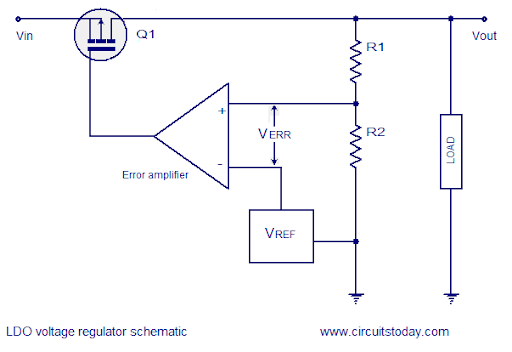
\includegraphics[width=\textwidth]{images/Gen_Linear_Voltage_Regulator.png}
    \label{fig:general-linear-voltage-regulator}
\end{figure}
\begin{figure}[H]
    \caption{LM7805 Pin Diagram}
    \centering
    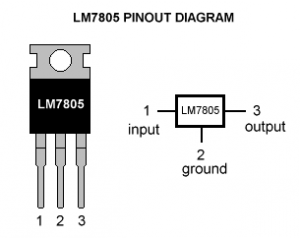
\includegraphics[width=\textwidth]{images/LM7805_pin_diagram.png}
    \label{fig:LM7805-pin-diagram}
\end{figure}
Just as any electrical device, linear voltage regulators will have their advantages and disadvantages. Linear voltage regulators are highly integrated devices. They are simple, cheap, responsive to changes in input voltage, load voltage, and there is no switching noise. Unlike linear voltage regulators, other voltage conversion circuits will have high-frequency switching noise, which may cause problems in the power system. Linear voltage regulators don’t have to worry about that issue. The biggest disadvantage is that they are inefficient. This inefficiency is due to the voltage drop across the active pass device and causes the regulator to produce a lot of heat.\par
Just as voltage regulators can be broken up into linear and switching voltage regulators, linear voltage regulators can be broken down into different types as well. There are two main types of linear voltage regulators: series voltage regulator and shunt voltage regulator. The main difference between the two is that with a series regulator, the active pass device is connected in series where in a shunt regulator it is connected in parallel. \par
As the name suggests for a series voltage regulator, the pass element in the circuit will be connected in series with the load, as shown in the figure below. Looking at the circuit, the output voltage is sensed through the voltage divider network in R1 and R2, and is compared to the VREF. As a result, the voltage drop across the transistor can be varied to make sure that the voltage across the load is constant. \par
\begin{figure}[H]
    \caption{Series Voltage Regulator}
    \centering
    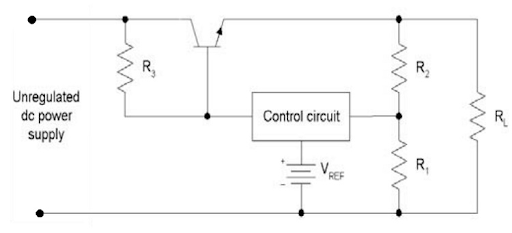
\includegraphics[width=\textwidth]{images/Series_Voltage_Regulator.png}
    \label{fig:series-voltage-regulator}
\end{figure}
The main advantages to this type of linear voltage regulator is that the current is effectively used by the load. This makes it more efficient than shunt voltage regulators. Regardless, the efficiency is still low compared to a switching voltage regulator but it is simple and the output will not have any switching spikes.\par
The figure below shows the circuit schematic of a shunt voltage regulator. The pass element in the circuit is connected in parallel while the resistors are connected the same as in the series voltage regulator. For this voltage regulator, voltage is maintained through the current drawn through the resistors and as the current is varied, the output voltage across the load remains constant. \par
\begin{figure}[H]
    \caption{Shunt Voltage Regulator}
    \centering
    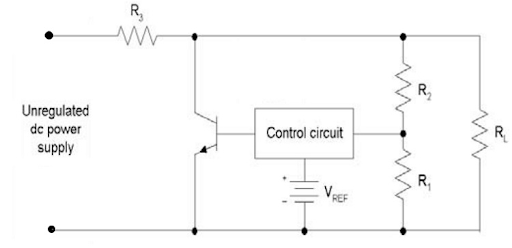
\includegraphics[width=\textwidth]{images/Shunt_Voltage_Regulator.png}
    \label{fig:shunt-voltage-regulator}
\end{figure}
When compared to the series voltage regulator, it is just slightly less efficient, but is simpler to implement into the circuit. This type of linear voltage regulator is less common and is used commonly in low-powered circuits and in voltage reference circuits.\par
\subparagraph{Switching Voltage Regulator}
Switching voltage regulators is a type of regulator that acts as a switch, where input power is turned on until the desired voltage is reached. After the desired voltage is reached, the switch element is turned off and stops any input power from coming in. With this type of voltage regulator, switching noise occurs because of the high-frequency from the reference voltage and the amplifier. As a result of the noise, capacitors, inductors, and other electrical components are used to smoothen out and reduce the noise. Regardless of the noise that occurs with switching voltage regulators, this type still remains very efficient because of the process of switching on and off at such high speeds. As said before, this type of regulator repeats its operation at high speeds, which allows it to supply voltage more efficiently and reduce heat generation. The figures below will show what the general schematic of a switching voltage regulator looks like but also the pin-out diagram for a lm2596 voltage regulator. You can see the difference in how many pins the lm2596 voltage regulator and the lm7805 voltage regulator. That is because switching voltage regulators require two more pins for the switch element as well as the feedback.\par
\begin{figure}[H]
    \caption{General Switching Voltage Regulator}
    \centering
    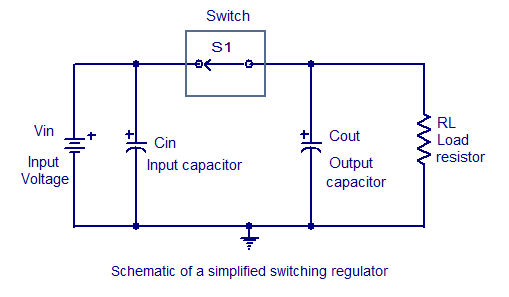
\includegraphics[width=\textwidth]{images/Gen_Switching_Voltage_Regulator.png}
    \label{fig:general-switching-voltage-regulator}
\end{figure}
\begin{figure}[H]
    \caption{LM2596 Pin Diagram}
    \centering
    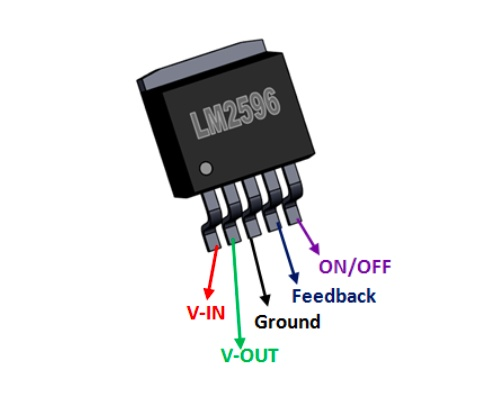
\includegraphics[width=\textwidth]{images/LM2596_pin_diagram.png}
    \label{fig:lm2596-pin-diagram}
\end{figure}
Some advantages to this type of voltage regulator is that it has a much higher efficiency, it does not produce a lot of heat, and it is capable of higher power efficiencies. The downside to this is that it has a more complex design, produces more noise which will require it to have more external components added to the circuit design. The choice between linear and switching voltage regulators always depends on what it is being used for because each design requires different things but switching voltage regulators are also a popular choice because of how efficient they are with power input and its general efficiency.\par
There are 3 main types of switching voltage regulators: buck converter, boost converter, and buck/boost converter. These three types of voltage regulators perform similar actions but all produce different output voltages.\par
Buck converters, also known as step-down converters, will lower the output voltage than the input voltage. This is similar to linear voltage regulators because linear voltage regulators work to make sure the output voltage is always lower than the input. The difference is that there will be less waste. The figure below shows the circuit schematic of a buck converter. Normally, a transistor is used as the switching element, connecting and disconnecting the input voltage to the inductor. \par
\begin{figure}[H]
    \caption{Buck Converter (Step Down) Circuit Schematic}
    \centering
    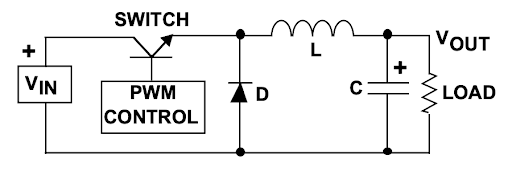
\includegraphics[width=\textwidth]{images/Buck_Converter.png}
    \label{fig:buck-converter-schematic}
\end{figure}
Boost converters, also known as step-up converters, will provide a higher output voltage than the input voltage. Even though the output voltage can be higher than the input voltage, the power being provided still has to be regulated within the output power specification of the circuit. Figure 8 shows the circuit schematic of the boost converter. As shown, the components are switched around compared to the buck converter. This allows the output voltage to increase, because when the switch is on, the voltage has to go across the inductor, increasing the current. When the switch is off, the diode is forward biased and charges the load higher than the input.\par
\begin{figure}[H]
    \caption{Boost Converter (Step Up) Circuit Schematic}
    \centering
    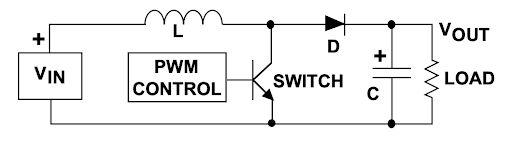
\includegraphics[width=\textwidth]{images/Boost_Converter.png}
    \label{fig:boost-converter-schematic}
\end{figure}
The last type is the buck/boost converter and as the name suggests, this type of converter is able to supply either a larger or smaller output voltage, but can also invert the polarity. This type of voltage regulator is common with battery operated products because at first use the battery will supply full power but throughout time the battery as well as input power will depreciate. Figure 9 shows the circuit schematic of the buck/boost converter. This converter operates similarly to both the buck converter and the boost converter but differs because it is capable of inverting the polarity. This is done by forward-biasing the reverse-biased diode when the switch is off. \par
\begin{figure}[H]
    \caption{Buck/Boost Converter Circuit Schematic}
    \centering
    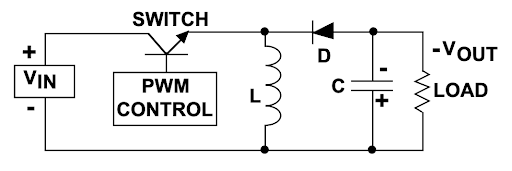
\includegraphics[width=\textwidth]{images/Buck_Boost_Converter.png}
    \label{fig:buck-boost-schematic}
\end{figure}
This type of converter offers many benefits. One of the reasons that it offers so much is because it brings both the buck converter and the boost converter together. It also offers lower operation cycling and is more efficient between the input and output voltages. A few downsides to this is that there is no isolation between the input and output and the output is always inverted, which results in complex sensing and feedback in the circuit. \par
\subparagraph{Voltage Regulator Selection}
The main function of a voltage regulator is to regulate output voltage from the power source, which is the 12V battery powered by solar panels, to the microcontroller and other components, ensuring that each part receives the correct amount of voltage. The microcontroller we will be using, the Texas Instruments CC3200, operates at a 3.3V input voltage and as a result will require a voltage regulator that can lower the output voltage. \par
As mentioned before, not all components are going to have the same operating voltages. With the various components and voltage requirements, multiple types of voltage regulators will be tested to see which one will be the most efficient and best fit for our model.\par
For our system, we will be looking at the LD1117 series (Linear), LM317 (Linear), LM2576 (Switching), and LM2596 (Switching). Of the various types of regulators, these were picked because the required input voltage for the CC3200 is 3.3V. These different voltage regulators will be compared based on efficiency, output voltage, cost, and any other feature that it may offer. \par
From the datasheets of each voltage regulator we were able to make the comparisons in the table below.\par
\begin{table}[H]
    \centering
	\begin{tabularx}{\textwidth}
			{
			| >{\raggedright\arraybackslash}X
			| >{\raggedright\arraybackslash}X
			| >{\raggedright\arraybackslash}X
			| >{\raggedright\arraybackslash}X
			| >{\raggedright\arraybackslash}X
			|
		}
		\caption{Voltage Regulators}
		\label{table:voltageregulators} \\
		\hline
		\textbf{Feature} & \textbf{LD1117\-series} & \textbf{LM317} & \textbf{LM2576} &  \textbf{LM2596} \\
		\hline
		\textbf{Voltage\-Regulator Type} & Linear & Linear & Switching & Switching \\
		\hline
		\textbf{Operating Voltage} & 15V  & 3V - 40V & 3V - 40V & 4.5V - 40V \\
		\hline
		\textbf{Output Voltage} & 3.3V & 1.25V - 37V & 3.3V, 5V, 12V,\-15V & 3.3V, 5V, 12V \\
		\hline
		\textbf{Output Option} & Fixed & Adjustable & Adjustable & Adjustable \\
		\hline
		\textbf{Operating Temp} & 0$^{\circ}$C - 125$^{\circ}$C & 0$^{\circ}$C - 125$^{\circ}$C  &  -40$^{\circ}$C - 125$^{\circ}$C & -40$^{\circ}$C - 125$^{\circ}$C \\
		\hline
		\textbf{Efficiency} & $\leq$62\% & Varies & 75\% & 73\% \\ 
		\hline
		\textbf{Frequency} & N/A & N/A & 53kHz & 150kHz \\
		\hline
		\textbf{Cost (\$)} & \$0.90 & \$0.99 & \$3.69 & \$6.73 \\
		\hline
	\end{tabularx}
\end{table}
Through comparison, it was agreed upon to select the LM317 (linear) and the LM2576 (switching) because of what was given to us by the datasheets. These were also selected so that we can observe and compare them even further to see which one will perform the best and be a good fit for our model.\par
\subsubsection{Sensing Subsystem}

The sensing subsystem will consist of a Visible / Near Infrared Spectrometer.

The spectrometer will consist of several optical, electrical and mechanical components:
    \begin{itemize}
        \item Silicon Photodiode
        \item Near Infrared Spectrum InGaAs Photodiode
        \item Linear Stage Actuator Carriage Rail
        \item Reflective Diffraction Grating
        \item Focusing Optic
        \item Fiber Patch Cable with attached Collimator
        \item LED Diode Array
    \end{itemize}

	\paragraph{Silicon Photodiode}

	The silicon photodiode will be one of the two detectors in the system, responsible for covering the visible spectrum of the soil emissions. Silicon photodiodes are cheap and overdeveloped for this application, much of the marketing emphasizes high speed current rise times and low dark current. Our spectrometer will not require either. Instead, it will be useful to have a detector with large surface area. This will reduce the precision required of other optical elements in the system, while retaining the flexibility to reduce the active area of the detector with a small aperture if needed. As always, low cost will be favored.


\begin{table}[H]
	\centering
	\label{table:SiliconPhotodiodes}
	\caption{Silicon Photodiodes}
	\begin{tabular}{|l|l|l|l|l|l|}
	\hline
	Manufacturer & Model & Range (nm) & Area (mm squared) & Dark Current (nA) & Cost (\textdollar)\\
    \hline
	Newark & BPX 61 & 400-1100 & 7.02 & 2 & 13.06\\
    \hline
	Digikey & ODD-1B & 400-1100 & 1 & 0.2 & 15.60\\
    \hline
	Digikey Opto Diode Corp & ODD-5W & 300-1100 & 5 & 1 & 14.50\\
    \hline
	Edmund Optics & PIN-3CD	350-1100 & 3.2 & 0.15 & 34.00\\
    \hline
	Thorlabs & FD11A & 320-1100 & 1.21 & 0.002 & 15.69\\
    \hline
	Thorlabs & FDS100 & 350-1100 & 13 & 1 & 16.08\\
    \hline
	\end{tabular}
\end{table}


The BPX 61 by Newark has a substantially better size to cost ratio than other relevant devices on the market, however it also has a higher ambient current than all others. One option is to select it and then compensate by investing in more LEDs to illuminate the target area and boost the signal up over the higher dark current, or by investing in more circuitry to clean up and boost the signal. Another option is to forgo the larger surface area and choose the sensor with the least ambient noise, Thorlabs’ FD11A. There don’t appear to be any standout choices aside from those two. All the other devices make compromises between their specs, while these two have standout specs, but require compromises in design. The BPX 61 offers the greatest flexibility, so it’s our choice for the visible-spectrum photodiode.

\paragraph{Near Infrared Spectrum InGaAs Photodiode}

The NIR InGaAs photodiode is responsible for detecting the majority of the spectral area of interest in this soil spectrometer. Once again, the relevant specs are active area, cost, and dark current. Most NIR photodetectors are designed for highspeed free space optical communication, but this application very forgiving in terms of sensor speeds. 


\begin{table}[H]
	\centering
	\label{table:InGaAsPhotodiodes}
	\caption{InGaAs Photodiodes}
	\begin{tabular}{|l|l|l|l|l|l|}
	\hline
	Manufacturer & Model & Range (nm) & Area (mm squared) & Dark Current (nA) & Cost (\textdollar)\\
	\hline
	Digikey Excelitas & C30617BH & 800-1700 & 0.1 & 1 & 43.58\\
	\hline
	Digikey Advanced Photonix & 0800-3111-011 & 800-1700 & 1.36 & 0.2 & 50.21\\
	\hline
	Thorlabs & FGA015 & 800-1700 & 0.018 & 0.5 & 63.00\\
	\hline
	Thorlabs & FGA01 & 800-1700 & 0.01 & 0.05 & 67.55\\
	\hline
	Edmund Optics & N/A & 800-1700 & 0.07 & 0.03 & 88.00\\
	\hline
	Edmund Optics & N/A & 800-1700 & 0.12 & 0.05 & 88.00\\
	\hline
	Edmund Optics & N/A	800-1700 & 0.3 & 0.3 & 94.00\\
	\hline
	Edmund Optics & N/A & 800-1700 & 0.4 & 0.4 & 94.00\\
	\hline
	\end{tabular}
\end{table}

The Advanced Photonix 0800-3111-011, distributed by Digikey has the highest active area, the second lowest cost, and an acceptable midrange dark current. This makes it the obvious choice for the system’s NIR detector.

\paragraph{Linear Stage Actuator Carriage Rail}

There are several methods of detecting broad spectral regimes. Scanning is much more viable than staring in this case, since staring detection requires an array of detectors. This system is intended to keep costs low for the target user, and detectors are a disproportionately expensive part. Instead, this system will have a pair of detectors mounted on a carriage which will pass through the spatially separated beams of light. There are several important criteria for this part. It must be able to take small, precise, increment steps in order for the detectors to capture the soil emission with high resolution. It must have sufficient range of motion to cover the whole spectral range, from 400nm to 1700nm. And it must meet the size, weight, and power constraints imposed by the rest of the system. 


\begin{table}[H]
	\centering
	\label{table:LinearStageActuators}
	\caption{Linear Stage Actuator}
	\begin{tabular}{|l|l|l|l|l|l|l|l|}
	\hline
	Manufacturer & Model & Stroke Length (mm) & Step Angle (degrees) & Step Size (mm) & Voltage (V) & Current (A) & Cost (\textdollar)\\
	\hline
	Rattmmotor & T0601-50 & 50 & 1.8 & 0.005 & 24 & 0.8 & 39.00\\
	\hline
	TOAUTO & T0601-100 & 100 & 1.8 & 0.005 & 24 & 0.6 & 67.00\\
	\hline
	TOAUTO & T0601-101 & 50 & 1.8 & 0.005 & 24 & 0.6 & 89.00\\
	\hline
	Zeberoxyz & SFU1605 & 200 & 1.8 & 0.025 & N/A & 1.5 & 83.89\\
	\hline
	\end{tabular}
\end{table}

The ratio between the stroke length and step size needs to be well above 1,500 in order to meet the criterion for spectral resolution. Luckily, the product with the least range is well over that limit, at 10,000:1. That allows cost to become the driving factor. The T0601-50, distributed by Rattmmotor, is just over half the price of the next cheapest option. This is the group’s choice of scanner


\paragraph{Reflective Diffraction Grating}

Diffraction is the operating principle behind the spectrometer. The soil emissions will be composed of different wavelengths representing the chemical structure of the soil, and this will be increased under illumination and then separated by diffraction. A diffraction grating separates incident electromagnetic waves of different frequencies by confining them into a tightly bounded region on reflection or transmission. This confinement causes the waves to disperse, like a prism would, with waves of higher frequencies experiencing greater dispersion. Transmission gratings will not be very effective for weak signal diffraction, as in this application, because most of the optical power is concentrated straight through and not separated at all, with only weaker orders fully separating. Reflective diffraction gratings will provide the best efficiency for soil spectroscopy. In order to prevent the beam from diffracting so far that it reflects straight back into itself, where it cannot be collected, it will be necessary to acquire a diffraction grating with grooves which are blazed at an angle, so that the surface normal of the grating has a greater angle than 90 degrees. The blaze angle corresponding to the 1000 nm diffraction regime will suffice. Next, it will be necessary to calculate the angular spread of diffraction from 400nm to 1700nm off a diffraction grating from several incident angles. The first order diffraction must not overlap with the incident beam if it is to be measured. Increased size is also desirable, in order to maximize the number of wave-groove interactions and boost diffraction efficiency. 

\begin{table}[H]
	\centering
	\label{table:DiffractionGratings}
	\caption{Diffraction Gratings}
	\begin{tabular}{|l|l|l|l|l|l|}
	\hline
	Manufacturer & Model & Density lines/mm & Dimensions (mm) & Blaze Angle (nm) & Cost (\textdollar)\\
	\hline
	Thorlabs & GR13-0610 & 600 & 12.7x12.7x6 & 1000 & 76.58\\
	\hline
	Thorlabs & GR25-1210 & 1200 & 25x25x6 & 1000 & 125.77\\
	\hline
	Edmund optics & Stock 43-745 & 600 & 12.7x12.7x6 & 1000 & 80.00\\
	\hline
	Edmund optics & Stock 43-753 & 1200 & 12.7x12.7x6 & 1000 & 80.00\\
	\hline
	MKS Newport & 33025FL01-520R & 600 & 12.5x12.5x6 & 1000 & 155.00\\
	\hline
	MKS Newport & 33025FL01-530R & 1200 & 12.5x12.5x7 & 1000 & 155.00\\
	\hline
	ScienceTech	631-0024 & 1200 & 50x50x9.5mm & 1000 & 500.00\\
	\hline
	\end{tabular}
\end{table}

The spectral regime is too wide to be able to reliably use a 600 nm grating without losing information in the infrared. Unfortunately, efficiency is not a variable that can be compared from product to product, since it varies with wavelength and per polarization. This means the only remaining comparison is the ratio from cost to active area. ScienceTech can be ruled out immediately. Its cost to size ratio is not far from the other 1200 nm gratings on this list, but it would be difficult to justify doubling the project budget in order to achieve a marginal increase in grating power efficiency. This spec can also be compensated by cranking up the optical power probing the soil, presumably for less than the \textdollar45 difference between the Edmund Optics and Thorlabs models.


\paragraph{Focusing Optic (placeholder)}

Fiber Patch Cable with attached Collimator (placeholder)

\paragraph{LED Diode Array (placeholder)}


